\documentclass[aspectratio=169,10pt]{beamer}
%
% ════════════════════════════════════════════════════════════════════════════
\section{Our Modifications}

\begin{frame}[plain]
  \centering
  \vspace{1.2cm}
  {\Huge \textbf{Our Modifications}}\\[8pt]
  {\Large KMA \quad DKMA \quad GNN-KMA}
\end{frame}

% ════════════════════════════════════════════════════════════════════════════
\subsection{KMA: Kernelized Memetic Algorithm}
\useinnertheme{rectangles}

\definecolor{darkblue}{RGB}{10,36,99}
\definecolor{midblue}{RGB}{30,80,160}
\definecolor{accentblue}{RGB}{65,135,210}
\definecolor{lightgray}{RGB}{245,245,250}
\definecolor{alertred}{RGB}{180,30,30}
\definecolor{successgreen}{RGB}{20,130,80}
\definecolor{warnorange}{RGB}{200,100,20}

\setbeamercolor{palette primary}{bg=darkblue,fg=white}
\setbeamercolor{palette secondary}{bg=midblue,fg=white}
\setbeamercolor{palette tertiary}{bg=accentblue,fg=white}
\setbeamercolor{palette quaternary}{bg=darkblue,fg=white}
\setbeamercolor{structure}{fg=darkblue}
\setbeamercolor{frametitle}{bg=darkblue,fg=white}
\setbeamercolor{title}{bg=darkblue,fg=white}
\setbeamercolor{block title}{bg=midblue,fg=white}
\setbeamercolor{block body}{bg=lightgray,fg=black}
\setbeamercolor{block title alerted}{bg=alertred,fg=white}
\setbeamercolor{block body alerted}{bg=lightgray,fg=black}
\setbeamercolor{block title example}{bg=successgreen,fg=white}
\setbeamercolor{block body example}{bg=lightgray,fg=black}
\setbeamercolor{section in head/foot}{bg=darkblue,fg=white}
\setbeamercolor{subsection in head/foot}{bg=midblue,fg=white}
\setbeamercolor{itemize item}{fg=midblue}
\setbeamercolor{itemize subitem}{fg=accentblue}
\setbeamercolor{enumerate item}{fg=midblue}

% ─── Packages ─────────────────────────────────────────────────────────────────
\usepackage{amsmath,amssymb,amsfonts}
\usepackage{tikz}
\usetikzlibrary{shapes.geometric,arrows.meta,positioning,fit,calc,shadows}
\usepackage{pgfplots}
\pgfplotsset{compat=1.18}
\usepackage{booktabs}
\usepackage{tabularx}
\usepackage{xcolor}
\usepackage{fontawesome5}
\usepackage{hyperref}
\usepackage{multicol}
\usepackage{tcolorbox}
\tcbuselibrary{skins,breakable}
% bibliography handled via thebibliography inline

% ─── Custom tcolorbox styles ──────────────────────────────────────────────────
\tcbset{
  mybox/.style={
    enhanced,colback=lightgray,colframe=midblue,
    fonttitle=\bfseries\small,coltitle=white,
    attach boxed title to top left={yshift=-2mm,xshift=4mm},
    boxed title style={colback=midblue},
    boxrule=0.4pt,arc=2pt,
  },
  algbox/.style={
    enhanced,colback=blue!5,colframe=darkblue,
    fonttitle=\bfseries\footnotesize,coltitle=white,
    attach boxed title to top left={yshift=-2mm,xshift=4mm},
    boxed title style={colback=darkblue},
    boxrule=0.6pt,arc=2pt,
  },
  greenbox/.style={
    enhanced,colback=green!5,colframe=successgreen,
    boxrule=0.5pt,arc=2pt,
  },
  orangebox/.style={
    enhanced,colback=orange!8,colframe=warnorange,
    boxrule=0.5pt,arc=2pt,
  },
}

% ─── Helpers ──────────────────────────────────────────────────────────────────
\newcommand{\highlight}[1]{\textcolor{midblue}{\textbf{#1}}}
\newcommand{\red}[1]{\textcolor{alertred}{\textbf{#1}}}
\newcommand{\green}[1]{\textcolor{successgreen}{\textbf{#1}}}
\newcommand{\orange}[1]{\textcolor{warnorange}{\textbf{#1}}}
\newcommand{\citenum}[1]{\textsuperscript{\tiny[#1]}}
\setbeamerfont{footnote}{size=\tiny}
\renewcommand{\footnotesize}{\tiny}

% ─── Metadata ─────────────────────────────────────────────────────────────────
\title[FVS: Algorithms, Datasets \& GNN Hybrids]{%
  \textbf{Feedback Vertex Set Problem}\\[4pt]
  {\large Algorithm Design, Dataset Generation, and GNN-Guided Hybrid Solvers}}
\subtitle{KMA · DKMA · GNN-KMA v1/v2/v3}
\author[Tawkir Aziz Rahman]{\textbf{Tawkir Aziz Rahman}}
\institute[Project 4-2]{CSE 4-2 Algorithm Project}
\date{\today}

% ─── Navigation dots ──────────────────────────────────────────────────────────
\setbeamertemplate{navigation symbols}{}
\setbeamertemplate{footline}{%
  \leavevmode\hbox{%
    \begin{beamercolorbox}[wd=.33\paperwidth,ht=2.25ex,dp=1ex,center]{author in head/foot}%
      \usebeamerfont{author in head/foot}\insertshortauthor
    \end{beamercolorbox}%
    \begin{beamercolorbox}[wd=.34\paperwidth,ht=2.25ex,dp=1ex,center]{title in head/foot}%
      \usebeamerfont{title in head/foot}\insertshorttitle
    \end{beamercolorbox}%
    \begin{beamercolorbox}[wd=.33\paperwidth,ht=2.25ex,dp=1ex,right]{date in head/foot}%
      \usebeamerfont{date in head/foot}\insertshortdate{}\hspace*{1em}
      \insertframenumber{} / \inserttotalframenumber\hspace*{1ex}
    \end{beamercolorbox}}%
  \vskip0pt%
}

% ─────────────────────────────────────────────────────────────────────────────
\begin{document}

% ════════════════════════════════════════════════════════════════════════════
%  TITLE
% ════════════════════════════════════════════════════════════════════════════
\begin{frame}[plain]
  \begin{tikzpicture}[remember picture, overlay]
    \fill[darkblue] (current page.north west) rectangle
      ([yshift=-0.55\paperheight]current page.north east);
    \fill[midblue] ([yshift=-0.55\paperheight]current page.north west) rectangle
      (current page.south east);
    % decorative nodes
    \foreach \x/\y/\r in {2/7/0.18, 5/6.8/0.13, 3.5/7.5/0.10,
                           13/7.2/0.15, 14.5/6.9/0.12, 12/7.6/0.10}{
      \fill[white,opacity=0.08] (\x,\y) circle (\r);
    }
  \end{tikzpicture}
  \vspace{0.8cm}
  \begin{center}
    {\color{white}\Large\bfseries Feedback Vertex Set Problem}\\[6pt]
    {\color{accentblue!80!white}\normalsize Algorithm Design, Synthetic Dataset Generation}\\
    {\color{accentblue!80!white}\normalsize \& GNN-Guided Hybrid Solvers}\\[14pt]
    {\color{white!70!blue}\small KMA $\cdot$ DKMA $\cdot$ GNN-KMA v1 / v2 / v3}\\[20pt]
    \hrule\vspace{6pt}
    {\color{white}\normalsize\bfseries Tawkir Aziz Rahman}\\
    {\color{white!80!blue}\small CSE 4-2 Algorithm Project $\cdot$ \today}\\[10pt]
    \begin{tabular}{cc}
      \href{https://github.com/TAR2003/Feedback_Vertex_Set_Problem_Algorithm_Project_4-2}{%
        \color{white}\faGithub~\texttt{GitHub Repository}} &
      \href{https://www.kaggle.com/datasets/tawkirazizrahman/fvs-synthetic-dataset-100k}{%
        \color{white}\faDatabase~\texttt{Kaggle Dataset (100K)}}
    \end{tabular}
  \end{center}
\end{frame}

% ─── Table of Contents ────────────────────────────────────────────────────────
\begin{frame}{Outline}
  \begin{multicols}{2}
    \tableofcontents
  \end{multicols}
\end{frame}

% ════════════════════════════════════════════════════════════════════════════
\section{Problem Overview}
% ════════════════════════════════════════════════════════════════════════════

\begin{frame}{Feedback Vertex Set — Problem Statement}
  \begin{columns}[T]
    \begin{column}{0.54\textwidth}
      \begin{block}{Definition}
        Given a graph $G=(V,E)$, find the \textbf{smallest} set
        $S \subseteq V$ such that $G \setminus S$ is \emph{acyclic}.\\[4pt]
        \textbf{Directed FVS (DFVS):} $G \setminus S$ is a DAG.
      \end{block}
      \vspace{4pt}
      \begin{alertblock}{NP-Hardness}
        FVS is NP-hard in general; it is one of Karp's original 21
        NP-complete problems \cite{karp1972}.
        DFVS is also NP-hard \cite{karp1972}.
      \end{alertblock}
      \vspace{4pt}
      \begin{block}{Parameterized Complexity}
        FVS is fixed-parameter tractable in $k$ (solution size):
        $O(4^k \cdot k! \cdot n^{O(1)})$ \cite{becker2000}.
        Modern kernelization yields a $O(k^2)$-vertex kernel
        \cite{thomasse2010}.
      \end{block}
    \end{column}
    \begin{column}{0.42\textwidth}
      \begin{center}
        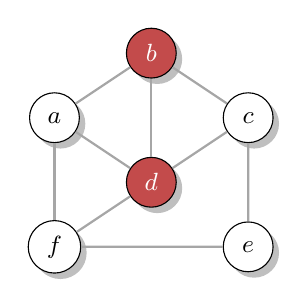
\begin{tikzpicture}[scale=0.82,
          every node/.style={circle,draw,minimum size=18pt,font=\small,
            fill=white,drop shadow},
          fvsnode/.style={fill=alertred!80,text=white},
          edge/.style={thick,gray!70}]
          \node (a) at (0,2)    {$a$};
          \node[fvsnode] (b) at (1.5,3)  {$b$};
          \node (c) at (3,2)    {$c$};
          \node[fvsnode] (d) at (1.5,1)  {$d$};
          \node (e) at (3,0)    {$e$};
          \node (f) at (0,0)    {$f$};
          \draw[edge] (a)--(b)--(c)--(d)--(a);
          \draw[edge] (b)--(d);
          \draw[edge] (c)--(e)--(f)--(d);
          \draw[edge] (a)--(f);
        \end{tikzpicture}\\[4pt]
        {\small\color{alertred}Red nodes $= $ FVS $\{b,d\}$}\\[2pt]
        {\tiny Removal leaves a forest}
      \end{center}
      \vspace{6pt}
      \begin{tcolorbox}[greenbox,fontupper=\footnotesize]
        \textbf{Applications:}\\
        Deadlock recovery, VLSI design,\\
        Bayesian network inference,\\
        circuit testing, bioinformatics
      \end{tcolorbox}
    \end{column}
  \end{columns}
\end{frame}

\begin{frame}{Project Scope \& Algorithm Hierarchy}
  \begin{center}
    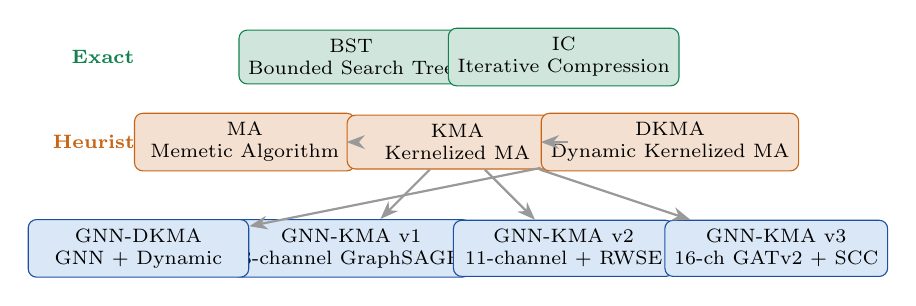
\begin{tikzpicture}[
      box/.style={rounded corners=3pt,draw,fill=blue!8,minimum width=2.8cm,
                  minimum height=0.6cm,font=\scriptsize,align=center},
      exactbox/.style={box,fill=successgreen!20,draw=successgreen},
      heurbox/.style={box,fill=warnorange!20,draw=warnorange},
      hybridbox/.style={box,fill=accentblue!20,draw=midblue},
      arr/.style={->,>=Stealth,thick,gray!80},
      scale=0.9]
      % Layer labels
      \node[font=\scriptsize\bfseries,text=successgreen] at (-3.5,1.7) {Exact};
      \node[font=\scriptsize\bfseries,text=warnorange]   at (-3.5,0.5) {Heuristic};
      \node[font=\scriptsize\bfseries,text=midblue]      at (-3.5,-1.0) {Hybrid ML};

      \node[exactbox]  (bst) at (0,1.7)   {BST\\Bounded Search Tree};
      \node[exactbox]  (ic)  at (3,1.7)   {IC\\Iterative Compression};
      \node[heurbox]   (ma)  at (-1.5,0.5) {MA\\Memetic Algorithm};
      \node[heurbox]   (kma) at (1.5,0.5)  {KMA\\Kernelized MA};
      \node[heurbox]   (dkma) at (4.5,0.5) {DKMA\\Dynamic Kernelized MA};
      \node[hybridbox] (g1)  at (0,-1.0)  {GNN-KMA v1\\3-channel GraphSAGE};
      \node[hybridbox] (g2)  at (3,-1.0)  {GNN-KMA v2\\11-channel + RWSE};
      \node[hybridbox] (g3)  at (6,-1.0)  {GNN-KMA v3\\16-ch GATv2 + SCC};
      \node[hybridbox] (gd)  at (-3,-1.0) {GNN-DKMA\\GNN + Dynamic};

      \draw[arr] (ma)--(kma);
      \draw[arr] (kma)--(dkma);
      \draw[arr] (kma)--(g1);
      \draw[arr] (kma)--(g2);
      \draw[arr] (kma)--(g3);
      \draw[arr] (dkma)--(gd);
    \end{tikzpicture}
  \end{center}
\end{frame}

% ════════════════════════════════════════════════════════════════════════════
\section{Exact Solvers}
% ════════════════════════════════════════════════════════════════════════════

\begin{frame}{Exact Solvers: BST \& IC}
  \begin{columns}[T]
    \begin{column}{0.47\textwidth}
      \begin{block}{Bounded Search Tree (BST)}
        \begin{itemize}\setlength\itemsep{2pt}
          \item Pick a cycle $C$; branch on every vertex of $C$
          \item At each branch, include that vertex in the FVS
          \item Prune when solution size $> k$
          \item Complexity: $O(4^k \cdot n)$ \cite{becker2000}
          \item Combined with \textbf{reduction rules}:
            self-loops, degree-1 bypass, degree-2 bypass
          \item Applicable only for small $k$ (exact track)
        \end{itemize}
      \end{block}
    \end{column}
    \begin{column}{0.47\textwidth}
      \begin{block}{Iterative Compression (IC)}
        \begin{itemize}\setlength\itemsep{2pt}
          \item Introduced by Reed et al.\ \cite{reed2004}
          \item Maintains a solution $S$ of size $k+1$;
            iteratively \textbf{compresses} to size $k$
          \item Uses important separator enumeration
          \item Yields $O(5^k \cdot k \cdot n^2)$ time \cite{cygan2015}
          \item Provides \textbf{exact labels} for
            GNN training on the exact track
          \item Correctness enforced via acyclicity
            check on final solution
        \end{itemize}
      \end{block}
    \end{column}
  \end{columns}
  \vspace{4pt}
  \begin{tcolorbox}[orangebox,fontupper=\footnotesize]
    \textbf{Usage in this project:} IC is used as the \textbf{label oracle} for
    exact-track GNN training data. BST is a secondary exact baseline.
    Both rely on the parameterized FVS kernel theory of Thomassé \cite{thomasse2010},
    which reduces any instance to a $O(k^2)$-vertex kernel.
  \end{tcolorbox}
\end{frame}

% ════════════════════════════════════════════════════════════════════════════
\section{Our Modifications}
% ════════════════════════════════════════════════════════════════════════════
\subsection{KMA: Kernelized Memetic Algorithm}

\begin{frame}{KMA — Motivation and High-Level Design}
  \begin{columns}[T]
    \begin{column}{0.52\textwidth}
      \textbf{Why not pure Memetic Algorithm?}
      \begin{itemize}
        \item A plain MA \cite{lust2010} operates on the full graph
        \item Reduction rules can \emph{safely} eliminate many vertices
          before any search \cite{thomasse2010}
        \item This shrinks the search space, letting MA focus on hard subgraphs
      \end{itemize}
      \vspace{6pt}
      \textbf{KMA Pipeline}
      \begin{enumerate}\setlength\itemsep{2pt}
        \item \highlight{Kernelization} — apply reduction rules, record forced vertices
        \item \highlight{MA on kernel} — C++ evolutionary search on reduced graph
        \item \highlight{Reconstruction} — map kernel solution to original indices,
          union with forced vertices
      \end{enumerate}
    \end{column}
    \begin{column}{0.44\textwidth}
      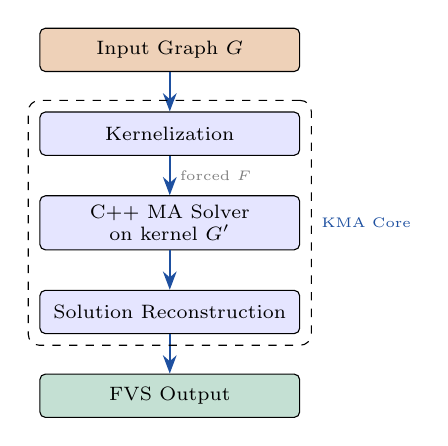
\begin{tikzpicture}[
        node distance=0.5cm,
        block/.style={draw,rounded corners=2pt,fill=blue!10,
                      minimum width=3.3cm,minimum height=0.55cm,
                      font=\scriptsize,align=center},
        arr/.style={->,>=Stealth,thick,midblue}]
        \node[block,fill=warnorange!30] (in)   {Input Graph $G$};
        \node[block,below=of in]  (kern) {Kernelization};
        \node[block,below=of kern](ma)   {C++ MA Solver\\on kernel $G'$};
        \node[block,below=of ma]  (recon){Solution Reconstruction};
        \node[block,below=of recon,fill=successgreen!25] (out) {FVS Output};
        \draw[arr] (in)--(kern);
        \draw[arr] (kern)--(ma) node[midway,right,font=\tiny,text=gray]
          {forced $F$};
        \draw[arr] (ma)--(recon);
        \draw[arr] (recon)--(out);
        \node[draw,dashed,rounded corners,fit=(kern)(ma)(recon),
              inner sep=4pt,label={[font=\tiny,midblue]right:KMA Core}]{};
      \end{tikzpicture}
    \end{column}
  \end{columns}
\end{frame}

\begin{frame}{KMA — Kernelization Rules}
  \begin{columns}[T]
    \begin{column}{0.47\textwidth}
      \begin{block}{Undirected Kernelization Rules}
        \begin{enumerate}\setlength\itemsep{3pt}
          \item \textbf{Self-loop:} vertex with self-loop $\Rightarrow$ force into FVS
          \item \textbf{Degree-0/1:} acyclic leaf $\Rightarrow$ safely delete
          \item \textbf{Degree-2 bypass:} if $\deg(v)=2$ with neighbors $a,b$
            and $\{a,b\}\notin E$:
            delete $v$, add edge $(a,b)$
        \end{enumerate}
        Rules applied \textbf{iteratively} until quiescence.\\[4pt]
        Theoretical basis: $O(k^2)$ kernel \cite{thomasse2010}.
      \end{block}
    \end{column}
    \begin{column}{0.47\textwidth}
      \begin{block}{Directed Kernelization Rules}
        \begin{enumerate}\setlength\itemsep{3pt}
          \item \textbf{Self-loop:} forced into DFVS
          \item \textbf{Source/Sink:} $\text{in-deg}=0$ or $\text{out-deg}=0$
            $\Rightarrow$ delete (not on any directed cycle)
          \item \textbf{Degree-1 bypass:} in-deg or out-deg $=1$
            $\Rightarrow$ shortcut edges, delete vertex
          \item \textbf{SCC reduction:} retain only vertices in
            nontrivial SCCs (size $>1$ or self-loop)
        \end{enumerate}
        Directed kernel theory: \cite{chen2008dfvs}.
      \end{block}
    \end{column}
  \end{columns}
  \vspace{4pt}
  \begin{tcolorbox}[greenbox,fontupper=\footnotesize]
    \textbf{Modification over baseline MA:} The addition of kernelization
    (especially the SCC-based directed reduction) is a key novelty.
    SCC reduction alone can eliminate \textbf{60--90\%} of vertices
    on sparse real-world directed graphs before any search begins.
  \end{tcolorbox}
\end{frame}

\begin{frame}{KMA — Memetic Algorithm Core}
  \begin{columns}[T]
    \begin{column}{0.50\textwidth}
      \textbf{C++ MA Solver} (evolutionary search on kernel):
      \begin{itemize}\setlength\itemsep{2pt}
        \item Initialise population of size $P$ randomly
        \item Each individual: binary vector over kernel vertices
        \item Each generation:
          \begin{enumerate}\setlength\itemsep{1pt}
            \item \textbf{Crossover} (two parents $\to$ offspring)
            \item \textbf{Local mutation} (flip, swap)
            \item \textbf{Repair}: restore FVS validity via greedy cycle cover
            \item \textbf{Selection}: tournament
          \end{enumerate}
        \item Early-stop if no improvement for $T$ generations
        \item Hard wall-clock timeout enforced inside C++
      \end{itemize}
      \vspace{4pt}
      Solver dispatch priority (best-first):
      \texttt{KMA} $\to$ \texttt{KME} $\to$ \texttt{MA}
    \end{column}
    \begin{column}{0.46\textwidth}
      \begin{block}{Parameters}
        \begin{tabular}{lll}
          \toprule
          Param & Flag & Default\\
          \midrule
          Population & \texttt{--pop} & 20\\
          Max generations & \texttt{--gens} & 100\\
          Timeout & \texttt{--timeout} & 600s\\
          Early-stop & \texttt{--earlystop} & 30\\
          \bottomrule
        \end{tabular}
      \end{block}
      \vspace{6pt}
      \begin{tcolorbox}[algbox,title=Complexity Note]
        \footnotesize
        Kernelization: $O(n+m)$ per pass\\
        MA on kernel $G'$: heuristic,\\
        ~~$O(P \cdot \text{gen} \cdot |V(G')|)$\\
        Full pipeline: practical for\\
        ~~$|V| \le 10^4$ within timeout
      \end{tcolorbox}
    \end{column}
  \end{columns}
\end{frame}

% ════════════════════════════════════════════════════════════════════════════
\subsection{DKMA: Dynamic Kernelized Memetic Algorithm}
% ════════════════════════════════════════════════════════════════════════════

\begin{frame}{DKMA — Core Idea}
  \begin{columns}[T]
    \begin{column}{0.52\textwidth}
      \textbf{Limitation of static kernelization (KMA):}
      \begin{itemize}
        \item Kernelization is applied \emph{once} before MA
        \item Partial solutions during MA may \emph{unlock} new reductions —
          these are never exploited
      \end{itemize}
      \vspace{4pt}
      \textbf{DKMA — Dynamic interleaving} \cite{pace2022,esa2022}:
      \begin{enumerate}\setlength\itemsep{2pt}
        \item Evolve population for one MA generation
        \item \highlight{Commit} vertices appearing in $\ge \tau$ fraction of individuals
        \item Force committed vertices into the solution
        \item \highlight{Re-kernelize} residual graph
        \item Continue MA on the smaller kernel
      \end{enumerate}
      \vspace{4pt}
      This \textbf{opening-up effect} progressively shrinks the kernel
      as partial agreement is reached.
    \end{column}
    \begin{column}{0.44\textwidth}
      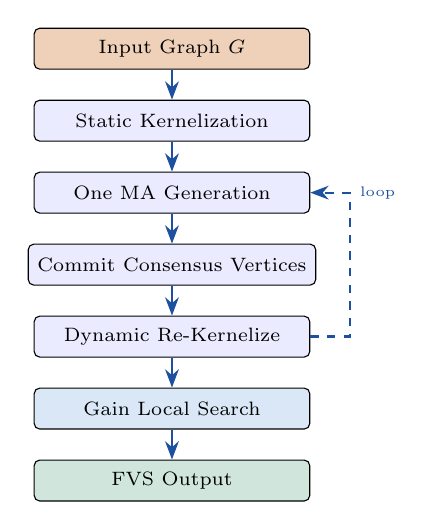
\begin{tikzpicture}[
        node distance=0.38cm,
        block/.style={draw,rounded corners=2pt,fill=blue!8,
                      minimum width=3.5cm,minimum height=0.52cm,
                      font=\scriptsize,align=center},
        loopback/.style={->,>=Stealth,thick,midblue,dashed},
        arr/.style={->,>=Stealth,thick,midblue}]
        \node[block,fill=warnorange!30] (in)   {Input Graph $G$};
        \node[block,below=of in]  (k1)   {Static Kernelization};
        \node[block,below=of k1]  (gen)  {One MA Generation};
        \node[block,below=of gen] (cmt)  {Commit Consensus Vertices};
        \node[block,below=of cmt] (rk)   {Dynamic Re-Kernelize};
        \node[block,below=of rk,fill=accentblue!20]  (ls)   {Gain Local Search};
        \node[block,below=of ls,fill=successgreen!20] (out) {FVS Output};
        \draw[arr] (in)--(k1);
        \draw[arr] (k1)--(gen);
        \draw[arr] (gen)--(cmt);
        \draw[arr] (cmt)--(rk);
        \draw[loopback] (rk.east) -- ++(0.5,0) |- (gen.east)
          node[midway,right,font=\tiny,text=midblue]{loop};
        \draw[arr] (rk)--(ls);
        \draw[arr] (ls)--(out);
      \end{tikzpicture}
    \end{column}
  \end{columns}
\end{frame}

\begin{frame}{DKMA — Key Innovations \& Helpers}
  \begin{columns}[T]
    \begin{column}{0.47\textwidth}
      \begin{block}{SHORTONE Directed Contractions}
        Inspired by the Mount-Doom PACE 2022 solver \cite{langedal2022},
        a directed contraction pass (\texttt{\_apply\_shortone\_rule})
        is applied before the MA loop on directed graphs.\\[3pt]
        Contracts degree-1 in/out vertices with special cycle-preserving rewiring,
        enabling additional SCC reductions.
      \end{block}
      \vspace{4pt}
      \begin{block}{Topological Diversification}
        Every 5 generations, \texttt{\_diversify\_with\_topological\_ordering}
        is called:\\
        \begin{itemize}
          \item Directed: randomised Kahn's algorithm tie-breaking
          \item Undirected: random spanning-tree cycle-breaking insertion
        \end{itemize}
        Prevents premature convergence \cite{lust2010}.
      \end{block}
    \end{column}
    \begin{column}{0.47\textwidth}
      \begin{block}{Gain Local Search (post-loop)}
        \texttt{\_gain\_local\_search} applies \textbf{1-1} and \textbf{2-1}
        improvement swaps after the MA loop:
        \begin{itemize}
          \item \textbf{1-1 swap}: remove one FVS vertex, add another
            if acyclicity is preserved and size decreases
          \item \textbf{2-1 swap}: replace two FVS vertices with one
        \end{itemize}
      \end{block}
      \vspace{4pt}
      \begin{block}{Commit Threshold \& Cap}
        \texttt{\_commit\_vertices\_from\_population}:
        \begin{itemize}
          \item Commit if vertex appears in $\ge \tau$ of population
          \item Cap at top 30\% by frequency if over-committing
          \item Default $\tau = 0.8$
        \end{itemize}
        Based on DFVS IPEC 2022 approach \cite{pace2022}.
      \end{block}
    \end{column}
  \end{columns}
\end{frame}

\begin{frame}{DKMA — Correctness \& Comparison with KMA}
  \begin{columns}[T]
    \begin{column}{0.44\textwidth}
      \begin{block}{Correctness Safeguards}
        \begin{itemize}\setlength\itemsep{2pt}
          \item Deduplicated final solution indices
          \item All forced vertices (static + dynamic) included
          \item Final \textbf{acyclicity verification} on original graph:
            directed $\Rightarrow$ iterative DFS back-edge detection;\\
            undirected $\Rightarrow$ union-find cycle check
          \item \red{Fallback to KMA} if validation fails
        \end{itemize}
      \end{block}
    \end{column}
    \begin{column}{0.52\textwidth}
      \begin{block}{KMA vs DKMA — Key Differences}
        \begin{tabular}{p{2.6cm}p{2.0cm}p{2.0cm}}
          \toprule
          Feature & KMA & DKMA\\
          \midrule
          Kernelization & Once & Per loop\\
          Commitment & None & Consensus\\
          SHORTONE pass & No & Yes (directed)\\
          Topological div. & No & Every 5 gen.\\
          Local search & No & Gain 1-1/2-1\\
          Acyclicity check & End & End + fallback\\
          \bottomrule
        \end{tabular}
      \end{block}
    \end{column}
  \end{columns}
  \vspace{4pt}
  \begin{tcolorbox}[orangebox,fontupper=\footnotesize]
    \textbf{References:} DKMA design is inspired by the PACE 2022 FVS track
    winner strategies \cite{pace2022} (Grossmann, Heuer, Schulz, Strash, IPEC 2022)
    and the ESA 2022 DFVS analysis \cite{esa2022}
    (Figiel, Froese, Nichterlein, Niedermeier).
    The Mount-Doom SHORTONE rule is from Langedal et al.\ \cite{langedal2022}.
  \end{tcolorbox}
\end{frame}

% ════════════════════════════════════════════════════════════════════════════
\subsection{GNN-KMA Models}
% ════════════════════════════════════════════════════════════════════════════

\begin{frame}{GNN-KMA — Hybrid Coupling Strategy}
  \begin{columns}[T]
    \begin{column}{0.50\textwidth}
      \textbf{Motivation:}
      \begin{itemize}
        \item GNN learns vertex-level patterns from solved instances
        \item Predicts probability $p(v)$ of belonging to FVS
        \item High-confidence predictions \textbf{hard-fix} vertices
          before KMA, reducing the search problem
      \end{itemize}
      \vspace{6pt}
      \textbf{Precision-first soft-hint coupling:}
      \begin{enumerate}\setlength\itemsep{2pt}
        \item Kernelize graph $G \to G'$
        \item Run GNN on $G'$, get $p(v)$ for each $v$
        \item Hard-fix only vertices with $p(v) \ge \theta$
        \item Cap hard-fix at \textbf{8\%} of kernel size
        \item Run KMA on residual kernel
        \item Reconstruct: forced $\cup$ GNN-fixed $\cup$ KMA output
      \end{enumerate}
      \vspace{3pt}
      {\footnotesize Default: $\theta=0.65$,
       min-fix $= 0.5\%$, max-fix $= 8\%$ of kernel}
    \end{column}
    \begin{column}{0.46\textwidth}
      \begin{tcolorbox}[mybox,title=Why Precision-First?]
        \footnotesize
        False positives in hard-fixing are \textbf{catastrophic}:
        a wrongly fixed vertex inflates the FVS size permanently
        within that branch. Capping at 8\% and requiring $\theta \ge 0.65$
        ensures the GNN only commits when highly confident.
        \\[4pt]
        If no vertex exceeds $\theta$, the system
        \textbf{falls back to pure KMA} automatically.
      \end{tcolorbox}
      \vspace{5pt}
      \begin{tcolorbox}[greenbox,fontupper=\footnotesize]
        \textbf{GNN-DKMA variant:} Same coupling, but
        the residual kernel is handed to DKMA instead of KMA,
        enabling dynamic re-kernelization atop GNN guidance.
      \end{tcolorbox}
    \end{column}
  \end{columns}
\end{frame}

% ─── GNN-KMA v1 ───────────────────────────────────────────────────────────────
\begin{frame}{GNN-KMA v1 — Baseline Architecture}
  \begin{columns}[T]
    \begin{column}{0.47\textwidth}
      \begin{block}{Feature Engineering (3 channels)}
        \textbf{Undirected:}
        \begin{itemize}
          \item Normalised degree $d(v)/d_{\max}$
          \item Clustering coefficient $c(v)$ \cite{watts1998}
          \item Normalised $\log$-degree
        \end{itemize}
        \textbf{Directed:}
        \begin{itemize}
          \item Normalised in-degree
          \item Normalised out-degree
          \item Normalised $\min(\text{in},\text{out})$-degree
        \end{itemize}
      \end{block}
      \vspace{4pt}
      \begin{tcolorbox}[algbox,title=Design Choice]
        \footnotesize
        Clustering coefficient \cite{watts1998} captures local cycle density —
        vertices with high $c(v)$ are strong FVS candidates.
        This is a well-established heuristic from the
        small-world network literature.
      \end{tcolorbox}
    \end{column}
    \begin{column}{0.47\textwidth}
      \begin{block}{Model Architecture}
        \textbf{UndirectedFVSNet:}
        \begin{itemize}
          \item 3-layer \textbf{GraphSAGE} message passing \cite{hamilton2017}
          \item BatchNorm + Dropout after each layer
          \item MLP classification head
          \item 2-class \texttt{log-softmax} output
        \end{itemize}
        \textbf{DirectedFVSNet:}
        \begin{itemize}
          \item Custom directed aggregation layer\\
            (separate in / out / self terms)
          \item 3 layers + BN + Dropout + MLP
          \item 2-class \texttt{log-softmax} output
        \end{itemize}
      \end{block}
      \vspace{2pt}
      \begin{block}{Training Objective}
        Weighted NLL loss $+$ cosine LR schedule.\\
        Checkpoint by \textbf{validation F1} score.
      \end{block}
    \end{column}
  \end{columns}
  \vspace{2pt}
  {\scriptsize\color{gray}
   GraphSAGE \cite{hamilton2017}: Hamilton et al., NeurIPS 2017.
   Labels: IC solver on exact track, KMA on heuristic track.}
\end{frame}

% ─── GNN-KMA v2 ───────────────────────────────────────────────────────────────
\begin{frame}{GNN-KMA v2 — Richer Structural Features}
  \begin{columns}[T]
    \begin{column}{0.47\textwidth}
      \begin{block}{Feature Engineering (11 channels)}
        \begin{enumerate}\setlength\itemsep{2pt}
          \item Degree-like channels (in/out/min or undirected)
          \item \textbf{RWSE} — Random Walk Structural Encoding
            \cite{dwivedi2021}\\
            {\footnotesize short-range return probabilities at steps
             $\{2,3,4\}$}
          \item \textbf{Motif counts}: triangle count,
            4-cycle participation, 4-clique style counts \cite{ahmed2015}
          \item \textbf{k-core number} $\kappa(v)$ \cite{batagelj2003}
        \end{enumerate}
      \end{block}
    \end{column}
    \begin{column}{0.47\textwidth}
      \begin{block}{Architecture \& Training}
        \textbf{UndirectedFVSNetV2 / DirectedFVSNetV2:}
        \begin{itemize}
          \item Same GraphSAGE-style backbone as v1
          \item Upgraded input: \texttt{in\_channels=11}
          \item Richer representation $\Rightarrow$ stronger
            structural discrimination
        \end{itemize}
        \vspace{4pt}
        \textbf{Training:} same NLL + cosine schedule;
        checkpoint by validation F1.
      \end{block}
      \vspace{4pt}
      \begin{tcolorbox}[algbox,title=Why These Features?]
        \footnotesize
        \textbf{RWSE} \cite{dwivedi2021}: captures short-range cycle
        return probability — directly relevant to FVS membership.\\[3pt]
        \textbf{k-core} \cite{batagelj2003}: vertices deep in dense
        cores are more likely to be in any FVS.\\[3pt]
        \textbf{Motif counts} \cite{ahmed2015}: triangle/4-cycle
        participation indicates cycle exposure.
      \end{tcolorbox}
    \end{column}
  \end{columns}
\end{frame}

% ─── GNN-KMA v3 ───────────────────────────────────────────────────────────────
\begin{frame}{GNN-KMA v3 — Attention-Based Precision Model}
  \begin{columns}[T]
    \begin{column}{0.47\textwidth}
      \begin{block}{Feature Engineering (16 channels)}
        \begin{itemize}\setlength\itemsep{2pt}
          \item Extended \textbf{RWSE} horizon: steps $\{2,3,4,6,8,12,16\}$
            \cite{dwivedi2021}
          \item \textbf{SCC-aware channels} for directed cycle structure
            (SCC size, SCC membership depth)
          \item Cycle-score interaction features
          \item Directional ratio features ($\text{in}/(\text{in}+\text{out})$)
          \item Reduced reliance on expensive motif channels
        \end{itemize}
      \end{block}
      \vspace{3pt}
      \begin{tcolorbox}[algbox,title=SCC Channels (Directed)]
        \footnotesize
        SCC decomposition \cite{tarjan1972} provides structural depth:
        vertices in large SCCs are more critical for DFVS.
        SCC-size and SCC-depth channels directly encode this.
      \end{tcolorbox}
    \end{column}
    \begin{column}{0.47\textwidth}
      \begin{block}{DirectedFVSNetV3 Architecture}
        \begin{itemize}\setlength\itemsep{2pt}
          \item Input projection layer
          \item \textbf{5 residual GATv2 blocks} \cite{brody2022}
          \item Separate \textbf{forward} and \textbf{reverse} message paths
          \item Per-layer fusion projections
          \item \textbf{Global readout context} concatenated to node embedding
          \item Single-logit output per node (sigmoid)
        \end{itemize}
      \end{block}
      \vspace{3pt}
      \begin{block}{v3 Training Innovations}
        \begin{itemize}
          \item \textbf{AsymmetricFVSLoss}: penalises false positives more
            strongly (precision-oriented)
          \item Warmup + cosine LR + \textbf{gradient clipping}
          \item Checkpoint metric: \textbf{topk-precision@8\%}
            (matches hard-fix cap)
          \item 200 epochs (vs 100 for v1/v2)
        \end{itemize}
      \end{block}
    \end{column}
  \end{columns}
\end{frame}

\begin{frame}{GNN-KMA — Feature \& Architecture Evolution Summary}
  \begin{center}
    \begin{tabular}{llll}
      \toprule
      \textbf{Aspect} & \textbf{v1} & \textbf{v2} & \textbf{v3}\\
      \midrule
      Feature channels & 3 & 11 & 16\\
      Degree features & \checkmark & \checkmark & \checkmark\\
      Clustering coeff.\ \cite{watts1998} & \checkmark & -- & --\\
      RWSE \cite{dwivedi2021} & -- & steps $\{2,3,4\}$ & steps $\{2..16\}$\\
      Motif counts \cite{ahmed2015} & -- & \checkmark & reduced\\
      k-core \cite{batagelj2003} & -- & \checkmark & --\\
      SCC channels \cite{tarjan1972} & -- & -- & \checkmark\\
      Backbone & GraphSAGE \cite{hamilton2017} & GraphSAGE & GATv2 \cite{brody2022}\\
      Depth & 3 layers & 3 layers & 5 residual blocks\\
      Bidirectional & No & No & Yes (fwd+rev)\\
      Global readout & No & No & Yes\\
      Loss & NLL & NLL & AsymmetricFVSLoss\\
      Checkpoint metric & Val F1 & Val F1 & topk-prec@8\%\\
      Epochs & 100 & 100 & 200\\
      \bottomrule
    \end{tabular}
  \end{center}
\end{frame}

% ════════════════════════════════════════════════════════════════════════════
\section{Results}
% ════════════════════════════════════════════════════════════════════════════
\begin{frame}[plain]
  \centering
  \vspace{1.0cm}
  {\Huge \textbf{Results}}\\[6pt]
  {\Large Synthetic Dataset \quad PACE 2022 \quad Evaluation}
\end{frame}

\begin{frame}{Notation \& Terms}
  \begin{itemize}
    \item \textbf{MA}: Memetic Algorithm — a genetic algorithm with local search
    \item \textbf{KMA}: Kernelized Memetic Algorithm — MA applied on a reduced kernel
    \item \textbf{DKMA}: Dynamic Kernelized Memetic Algorithm — KMA with iterative re-kernelization
    \item \textbf{GNN-KMA}: GNN-augmented KMA — GNN guides/fixes high-confidence vertices for KMA
  \end{itemize}
\end{frame}

\subsection{Synthetic Dataset}

\begin{frame}{Dataset — Design Goals \& Generation Pipeline}
  \begin{columns}[T]
    \begin{column}{0.52\textwidth}
      \textbf{Five design goals:}
      \begin{enumerate}\setlength\itemsep{2pt}
        \item \highlight{Controlled distribution} — fixed category proportions
        \item \highlight{Track-aware difficulty} — separate exact \& heuristic tracks
        \item \highlight{Reproducibility} — deterministic seeding throughout
        \item \highlight{Restartability} — safe reuse of existing files
        \item \highlight{Benchmark/train alignment} — PT datasets mirror
          TXT corpus structure
      \end{enumerate}
      \vspace{6pt}
      \textbf{Three-stage orchestration:}
      \begin{enumerate}
        \item \texttt{download\_real\_world.py}\\
          {\footnotesize NetworkX, PyG, OGB, SNAP sources}
        \item \texttt{generate\_synthetic.py}\\
          {\footnotesize Barabási–Albert, Watts–Strogatz, ER, grids, trees, DAGs}
        \item \texttt{dataset\_gen.py}\\
          {\footnotesize TXT $\to$ PyG Data objects with solver labels}
      \end{enumerate}
    \end{column}
    \begin{column}{0.44\textwidth}
      \begin{tcolorbox}[mybox,title=Directory Contract]
        \footnotesize
        \texttt{data/synthetic/}\\
        \quad\texttt{\{undirected|directed\}/}\\
        \quad\quad\texttt{\{exact\_track|heuristic\_track\}/}\\
        \quad\quad\quad\texttt{\{category\}/}\\
        \quad\quad\quad\quad\texttt{*.txt}
      \end{tcolorbox}
      \vspace{6pt}
      \begin{block}{Track Size Intent}
        \begin{tabular}{ll}
          \toprule
          Track & Node range\\
          \midrule
          exact\_track & $\approx 10$--$35$ nodes\\
          heuristic\_track & $\approx 100$--$5000$ nodes\\
          \bottomrule
        \end{tabular}
      \end{block}
      \vspace{4pt}
      \begin{tcolorbox}[greenbox,fontupper=\footnotesize]
        \textbf{Default:} 100K undirected + 100K directed\\
        exact ratio = 0.5, seed = 1337
      \end{tcolorbox}
    \end{column}
  \end{columns}
\end{frame}

\begin{frame}{Dataset — Category Distribution}
  \begin{columns}[T]
    \begin{column}{0.50\textwidth}
      \begin{block}{Undirected (uniform weights, 20\% each)}
        \begin{tabular}{lll}
          \toprule
          Category & Weight & Graph Model\\
          \midrule
          \texttt{real\_world}  & 20\% & NetworkX/PyG/OGB/SNAP\\
          \texttt{scale\_free}  & 20\% & Barabási–Albert \cite{barabasi1999}\\
          \texttt{small\_world} & 20\% & Watts–Strogatz \cite{watts1998}\\
          \texttt{random\_er}   & 20\% & Erdős–Rényi \cite{erdos1959}\\
          \texttt{grids\_trees} & 20\% & Grid + Random tree\\
          \bottomrule
        \end{tabular}
      \end{block}
    \end{column}
    \begin{column}{0.46\textwidth}
      \begin{block}{Directed (non-uniform weights)}
        \begin{tabular}{lll}
          \toprule
          Category & Weight\\
          \midrule
          \texttt{real\_world\_ego}  & 30\%\\
          \texttt{scale\_free}       & 20\%\\
          \texttt{random\_er}        & 20\%\\
          \texttt{directed\_grids}   & 15\%\\
          \texttt{dags}              & 15\%\\
          \bottomrule
        \end{tabular}
      \end{block}
    \end{column}
  \end{columns}
  \vspace{6pt}
  \begin{columns}[T]
    \begin{column}{0.50\textwidth}
      \begin{tcolorbox}[greenbox,fontupper=\footnotesize]
        \textbf{Real-world share:}\\
        Undirected: 20\% from real-world sources\\
        Directed: 30\% from ego-network sources\\[3pt]
        Sources: NetworkX built-ins, PyG datasets,
        OGB node property datasets, SNAP archives.
        Cached under \texttt{.cache/real\_graphs}.
      \end{tcolorbox}
    \end{column}
    \begin{column}{0.46\textwidth}
      \begin{tcolorbox}[algbox,title=Label Sources]
        \footnotesize
        \textbf{exact\_track}: IC solver labels\\
        (high-fidelity, near-optimal)\\[3pt]
        \textbf{heuristic\_track}: KMA labels\\
        (practical, large-instance behavior)
      \end{tcolorbox}
    \end{column}
  \end{columns}
\end{frame}

\begin{frame}{Dataset — Why This Dataset is Strong}
  \begin{columns}[T]
    \begin{column}{0.46\textwidth}
      \begin{block}{Diversity}
        \begin{itemize}\setlength\itemsep{2pt}
          \item \textbf{5 undirected families}: covers scale-free hubs,
            small-world clusters, random structure,
            regular grids/trees, and real topology
          \item \textbf{5 directed families}: adds ego networks and DAGs
          \item Both undirected and directed instances
          \item Two difficulty regimes (exact / heuristic)
        \end{itemize}
      \end{block}
      \vspace{4pt}
      \begin{block}{Scale}
        100K total undirected + 100K directed\\
        {\footnotesize (20K version also available on Kaggle)}\\[4pt]
        Largest publicly available FVS dataset
        with ground-truth labels to our knowledge.
      \end{block}
    \end{column}
    \begin{column}{0.50\textwidth}
      \begin{block}{Quality Guarantees}
        \begin{itemize}\setlength\itemsep{2pt}
          \item Each label validated via acyclicity check
          \item Subprocess timeout isolation for all solver calls
          \item CSV status ledger tracks
            completed / timeout / invalid outcomes
          \item Largest connected component extracted
          \item Compact integer relabelling applied
          \item No self-loops in edge lists
        \end{itemize}
      \end{block}
      \vspace{4pt}
      \begin{tcolorbox}[greenbox,fontupper=\footnotesize]
        \faDatabase~\textbf{Kaggle (100K):}\\
        \href{https://www.kaggle.com/datasets/tawkirazizrahman/fvs-synthetic-dataset-100k}{%
          \texttt{kaggle.com/.../fvs-synthetic-dataset-100k}}\\[4pt]
        \faDatabase~\textbf{Kaggle (20K):}\\
        \href{https://www.kaggle.com/datasets/tawkirazizrahman/fvs-synthetic-dataset-20k}{%
          \texttt{kaggle.com/.../fvs-synthetic-dataset-20k}}
      \end{tcolorbox}
    \end{column}
  \end{columns}
\end{frame}

% ════════════════════════════════════════════════════════════════════════════
\subsection{PACE 2022 Benchmark}
% ════════════════════════════════════════════════════════════════════════════

\begin{frame}{PACE 2022 Dataset — Real-World Benchmark Testing}
  \begin{columns}[T]
    \begin{column}{0.52\textwidth}
      \begin{block}{What is PACE 2022?}
        The \textbf{Parameterized Algorithms and Computational Experiments}
        (PACE) Challenge 2022 \cite{pace2022} focused on the
        \textbf{Feedback Vertex Set} problem.\\[5pt]
        It provided:
        \begin{itemize}
          \item 200 public undirected test instances
          \item Curated from real-world and synthetic sources
          \item Difficulty ranges from small exact to large heuristic
          \item Official solution checker for validation
          \item World-class solver implementations as baselines
        \end{itemize}
      \end{block}
    \end{column}
    \begin{column}{0.44\textwidth}
      \begin{block}{Usage in This Project}
        \begin{itemize}\setlength\itemsep{3pt}
          \item PACE 2022 instances stored under
            \texttt{data/pace2022/}
          \item \textbf{Protected from cleanup} — never deleted
            by \texttt{setup\_benchmark\_inputs.py}
          \item Benchmarked via \texttt{pacerun.sh}
            and \texttt{paceresults/}
          \item Used to evaluate \textbf{heuristic solvers}
            (KMA, DKMA, GNN-KMA v1/v2/v3)
            against real competition-grade instances
          \item PACE winner results in \texttt{pace2022\_winner.csv}
            used as comparison baseline
        \end{itemize}
      \end{block}
    \end{column}
  \end{columns}
  \vspace{4pt}
  \begin{tcolorbox}[orangebox,fontupper=\footnotesize]
    \textbf{Why PACE 2022?} Our synthetic dataset covers diverse graph families
    but may not capture the nuances of competition-curated real-world instances.
    PACE 2022 instances serve as a \emph{held-out real-world stress test}
    for heuristic solvers, enabling direct comparison with state-of-the-art
    PACE competitors \cite{pace2022}.
  \end{tcolorbox}
\end{frame}

% ════════════════════════════════════════════════════════════════════════════
\section{System Architecture}
% ════════════════════════════════════════════════════════════════════════════

\begin{frame}{End-to-End System Architecture}
  \begin{center}
  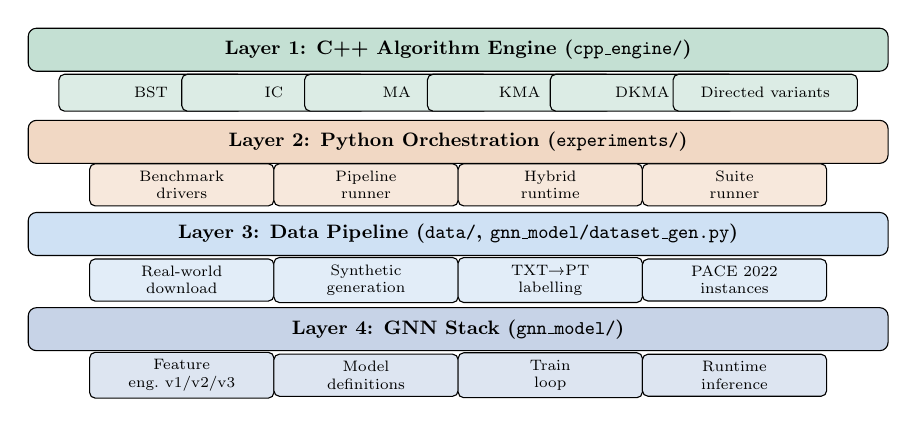
\begin{tikzpicture}[
    scale=0.78, transform shape,
    layer/.style={draw,fill=#1,rounded corners=3pt,
                  minimum width=14cm,minimum height=0.7cm,
                  font=\small\bfseries,align=center},
    module/.style={draw,fill=#1,rounded corners=2pt,
                   minimum width=3.0cm,minimum height=0.6cm,
                   font=\scriptsize,align=center},
    arr/.style={->,>=Stealth,thick,gray!70}]

    % Layer 1: C++ Engine
    \node[layer=successgreen!25] (cpp) at (0,3.6)
      {Layer 1: C++ Algorithm Engine (\texttt{cpp\_engine/})};
    \node[module=successgreen!15] (cppbst) at (-5,2.9) {BST};
    \node[module=successgreen!15] (cppic)  at (-3,2.9) {IC};
    \node[module=successgreen!15] (cppma)  at (-1,2.9) {MA};
    \node[module=successgreen!15] (cppkma) at ( 1,2.9) {KMA};
    \node[module=successgreen!15] (cppdkma)at ( 3,2.9) {DKMA};
    \node[module=successgreen!15] (cppdir) at ( 5,2.9) {Directed variants};

    % Layer 2: Python Orchestration
    \node[layer=warnorange!25] (pyorch) at (0,2.1)
      {Layer 2: Python Orchestration (\texttt{experiments/})};
    \node[module=warnorange!15] (bench) at (-4.5,1.4) {Benchmark\\drivers};
    \node[module=warnorange!15] (pipe)  at (-1.5,1.4) {Pipeline\\runner};
    \node[module=warnorange!15] (hybr)  at ( 1.5,1.4) {Hybrid\\runtime};
    \node[module=warnorange!15] (suite) at ( 4.5,1.4) {Suite\\runner};

    % Layer 3: Data
    \node[layer=accentblue!25] (data) at (0,0.6)
      {Layer 3: Data Pipeline (\texttt{data/}, \texttt{gnn\_model/dataset\_gen.py})};
    \node[module=accentblue!15] (rw)   at (-4.5,-0.15) {Real-world\\download};
    \node[module=accentblue!15] (syn)  at (-1.5,-0.15) {Synthetic\\generation};
    \node[module=accentblue!15] (pt)   at ( 1.5,-0.15) {TXT→PT\\labelling};
    \node[module=accentblue!15] (pace) at ( 4.5,-0.15) {PACE 2022\\instances};

    % Layer 4: GNN
    \node[layer=midblue!25] (gnn) at (0,-0.95)
      {Layer 4: GNN Stack (\texttt{gnn\_model/})};
    \node[module=midblue!15] (feat) at (-4.5,-1.7) {Feature\\eng.\ v1/v2/v3};
    \node[module=midblue!15] (mod)  at (-1.5,-1.7) {Model\\definitions};
    \node[module=midblue!15] (trn)  at ( 1.5,-1.7) {Train\\loop};
    \node[module=midblue!15] (inf)  at ( 4.5,-1.7) {Runtime\\inference};
  \end{tikzpicture}
  \end{center}
\end{frame}

% ════════════════════════════════════════════════════════════════════════════
\subsection{Results \& Evaluation}
% ════════════════════════════════════════════════════════════════════════════

\begin{frame}{Evaluation Framework}
  \begin{columns}[T]
    \begin{column}{0.50\textwidth}
      \begin{block}{Benchmark Output Format}
        Each benchmark run produces a CSV with:
        \begin{itemize}\setlength\itemsep{1pt}
          \item File identity \& graph metadata
          \item Algorithm / family / track tags
          \item \texttt{fvs\_size}: solution size
          \item \texttt{runtime}: wall-clock seconds
          \item \texttt{valid}: acyclicity-verified boolean
          \item \texttt{status}: completed / timeout / error
        \end{itemize}
      \end{block}
      \vspace{4pt}
      \begin{block}{Benchmark Tracks}
        \textbf{exact\_track:} compared against IC/BST optimal\\
        \textbf{heuristic\_track:} compared against MA baseline\\
        \textbf{PACE 2022:} compared against official winner
      \end{block}
    \end{column}
    \begin{column}{0.46\textwidth}
      \begin{block}{Algorithm Comparison Matrix}
        \begin{tabular}{lcc}
          \toprule
          Algorithm & Exact & Heuristic\\
          \midrule
          BST & \checkmark & --\\
          IC  & \checkmark & --\\
          MA  & -- & \checkmark\\
          KMA & -- & \checkmark\\
          DKMA & -- & \checkmark\\
          GNN-KMA v1 & -- & \checkmark\\
          GNN-KMA v2 & -- & \checkmark\\
          GNN-KMA v3 & -- & \checkmark\\
          GNN-DKMA  & -- & \checkmark\\
          \bottomrule
        \end{tabular}
      \end{block}
      \vspace{4pt}
      \begin{tcolorbox}[greenbox,fontupper=\footnotesize]
        \textbf{Resume semantics:} all benchmark
        pipelines support deterministic restart —
        interrupted runs continue from last completed file.
      \end{tcolorbox}
    \end{column}
  \end{columns}
\end{frame}

% ════════════════════════════════════════════════════════════════════════════
\section{Conclusions}
% ════════════════════════════════════════════════════════════════════════════

\begin{frame}{Summary \& Contributions}
  \begin{columns}[T]
    \begin{column}{0.47\textwidth}
      \begin{block}{\faCode~Algorithm Contributions}
        \begin{itemize}\setlength\itemsep{2pt}
          \item \highlight{KMA}: first-class kernelization (SCC reduction
            for directed; degree-2 bypass for undirected) integrated
            with C++ memetic search
          \item \highlight{DKMA}: dynamic re-kernelization loop,
            SHORTONE contractions \cite{langedal2022},
            topological diversification,
            gain local search (1-1 / 2-1 swaps)
          \item \highlight{GNN-KMA v1/v2/v3}: progressive feature and
            architecture improvements (GraphSAGE → GATv2 \cite{brody2022},
            3 → 16 channels, NLL → asymmetric precision loss)
          \item \highlight{GNN-DKMA}: GNN guidance + dynamic kernelization
        \end{itemize}
      \end{block}
    \end{column}
    \begin{column}{0.47\textwidth}
      \begin{block}{\faDatabase~Dataset Contributions}
        \begin{itemize}\setlength\itemsep{2pt}
          \item 100K undirected + 100K directed labelled FVS instances
          \item 5 graph families, 2 difficulty tracks, real+synthetic mix
          \item Solver-verified ground-truth labels (IC for exact,
            KMA for heuristic)
          \item Publicly released on Kaggle (100K and 20K versions)
          \item PACE 2022 integration for real-world benchmarking
        \end{itemize}
      \end{block}
      \vspace{4pt}
      \begin{tcolorbox}[greenbox,fontupper=\footnotesize]
        \faGithub~\textbf{GitHub:}\\
        {\tiny\url{https://github.com/TAR2003/Feedback_Vertex_Set_Problem_Algorithm_Project_4-2}}\\[4pt]
        \faDatabase~\textbf{Dataset (100K):}\\
        {\tiny\url{https://www.kaggle.com/datasets/tawkirazizrahman/fvs-synthetic-dataset-100k}}\\[2pt]
        \faDatabase~\textbf{Dataset (20K):}\\
        {\tiny\url{https://www.kaggle.com/datasets/tawkirazizrahman/fvs-synthetic-dataset-20k}}
      \end{tcolorbox}
    \end{column}
  \end{columns}
\end{frame}

% ════════════════════════════════════════════════════════════════════════════
%  REFERENCES
% ════════════════════════════════════════════════════════════════════════════
\begin{frame}[allowframebreaks]{References}
  \begin{thebibliography}{99}
    \scriptsize
    \bibitem{karp1972}
      R.M.~Karp,
      ``Reducibility among combinatorial problems,''
      in \emph{Complexity of Computer Computations}, 1972, pp.~85--103.

    \bibitem{becker2000}
      A.~Becker and D.~Geiger,
      ``Optimization of Pearl's method of conditioning and greedy-like approximation
       algorithms for the weighted maximum acyclic subgraph problem,''
      \emph{Artificial Intelligence}, vol.~105, pp.~1--2, 1996.

    \bibitem{thomasse2010}
      S.~Thomassé,
      ``A $4k^2$ kernel for feedback vertex set,''
      \emph{ACM Trans.\ Algorithms}, vol.~6, no.~2, 2010.

    \bibitem{reed2004}
      B.~Reed, K.~Smith, and A.~Vetta,
      ``Finding odd cycle transversals,''
      \emph{Operations Research Letters}, vol.~32, no.~4, 2004.

    \bibitem{cygan2015}
      M.~Cygan \emph{et al.},
      \emph{Parameterized Algorithms}.
      Springer, 2015.

    \bibitem{chen2008dfvs}
      J.~Chen, Y.~Liu, S.~Lu, B.~O'Sullivan, and I.~Razgon,
      ``A fixed-parameter algorithm for the directed feedback vertex set problem,''
      \emph{J.~ACM}, vol.~55, no.~5, 2008.

    \bibitem{lust2010}
      T.~Lust and J.~Teghem,
      ``The multiobjective multidimensional knapsack problem: a survey and a new approach,''
      \emph{Int.\ Trans.\ Oper.\ Res.}, 2010.
      {\footnotesize(Memetic algorithm framework reference.)}

    \bibitem{pace2022}
      G.~Grossmann, M.~Heuer, P.~Schulz, and D.~Strash,
      ``Targeted solution methods for the minimum feedback vertex set problem,''
      in \emph{Proc.\ 17th IPEC}, LIPIcs vol.~249, 2022,
      doi:10.4230/LIPIcs.IPEC.2022.26.

    \bibitem{esa2022}
      A.~Figiel, V.~Froese, A.~Nichterlein, and R.~Niedermeier,
      ``Improved parameterized algorithms for the directed feedback vertex set problem,''
      in \emph{Proc.\ ESA 2022}, LIPIcs, 2022,
      doi:10.4230/LIPIcs.ESA.2022.53.

    \bibitem{langedal2022}
      K.~Langedal, J.~Langguth, F.~Manne, and D.~Strash,
      ``Efficient minimum weight vertex cover heuristics using graph neural networks'' (Mount-Doom FVS solver),
      Zenodo, 2022, doi:10.5281/zenodo.6630611.

    \bibitem{hamilton2017}
      W.~Hamilton, Z.~Ying, and J.~Leskovec,
      ``Inductive representation learning on large graphs'' (GraphSAGE),
      in \emph{NeurIPS}, 2017.

    \bibitem{brody2022}
      S.~Brody, U.~Alon, and E.~Yahav,
      ``How attentive are graph attention networks?'' (GATv2),
      in \emph{ICLR}, 2022.

    \bibitem{dwivedi2021}
      V.P.~Dwivedi \emph{et al.},
      ``Benchmarking graph neural networks,''
      \emph{JMLR}, vol.~24, no.~43, 2023.
      {\footnotesize(RWSE/positional encoding reference.)}

    \bibitem{ahmed2015}
      N.K.~Ahmed, J.~Neville, R.A.~Rossi, and N.~Duffield,
      ``Efficient graphlet counting for large networks,''
      in \emph{ICDM}, 2015.

    \bibitem{batagelj2003}
      V.~Batagelj and M.~Zaversnik,
      ``An $O(m)$ algorithm for cores decomposition of networks,''
      \emph{arXiv:cs/0310049}, 2003.

    \bibitem{tarjan1972}
      R.E.~Tarjan,
      ``Depth-first search and linear graph algorithms,''
      \emph{SIAM J.~Comput.}, vol.~1, no.~2, 1972.

    \bibitem{barabasi1999}
      A.-L.~Barabási and R.~Albert,
      ``Emergence of scaling in random networks,''
      \emph{Science}, vol.~286, 1999.

    \bibitem{watts1998}
      D.J.~Watts and S.H.~Strogatz,
      ``Collective dynamics of `small-world' networks,''
      \emph{Nature}, vol.~393, 1998.

    \bibitem{erdos1959}
      P.~Erdős and A.~Rényi,
      ``On random graphs I,''
      \emph{Publicationes Mathematicae}, vol.~6, 1959.
  \end{thebibliography}
\end{frame}

% ─── Final slide ──────────────────────────────────────────────────────────────
\begin{frame}[plain]
  \begin{tikzpicture}[remember picture, overlay]
    \fill[darkblue] (current page.south west) rectangle (current page.north east);
  \end{tikzpicture}
  \begin{center}
    \vspace{1.8cm}
    {\color{white}\Huge\bfseries Thank You}\\[14pt]
    {\color{accentblue!80!white}\large Questions \& Discussion}\\[28pt]
    \hrule\vspace{10pt}
    \begin{tabular}{ll}
      \color{white}\faGithub & \color{white}{\small\url{https://github.com/TAR2003/Feedback_Vertex_Set_Problem_Algorithm_Project_4-2}}\\[6pt]
      \color{white}\faDatabase & \color{white}{\small\url{https://www.kaggle.com/datasets/tawkirazizrahman/fvs-synthetic-dataset-100k}}\\[6pt]
      \color{white}\faDatabase & \color{white}{\small\url{https://www.kaggle.com/datasets/tawkirazizrahman/fvs-synthetic-dataset-20k}}\\
    \end{tabular}
  \end{center}
\end{frame}

\end{document}